\documentclass[border=10pt]{standalone}
\usepackage[svgnames]{xcolor}
\usepackage{amsmath}
\usepackage{pgfplots}
\pgfplotsset{compat=newest}
\usepackage[sfdefault]{FiraSans}
\usepackage{FiraMono}
\renewcommand*\familydefault{\sfdefault}
\begin{document}
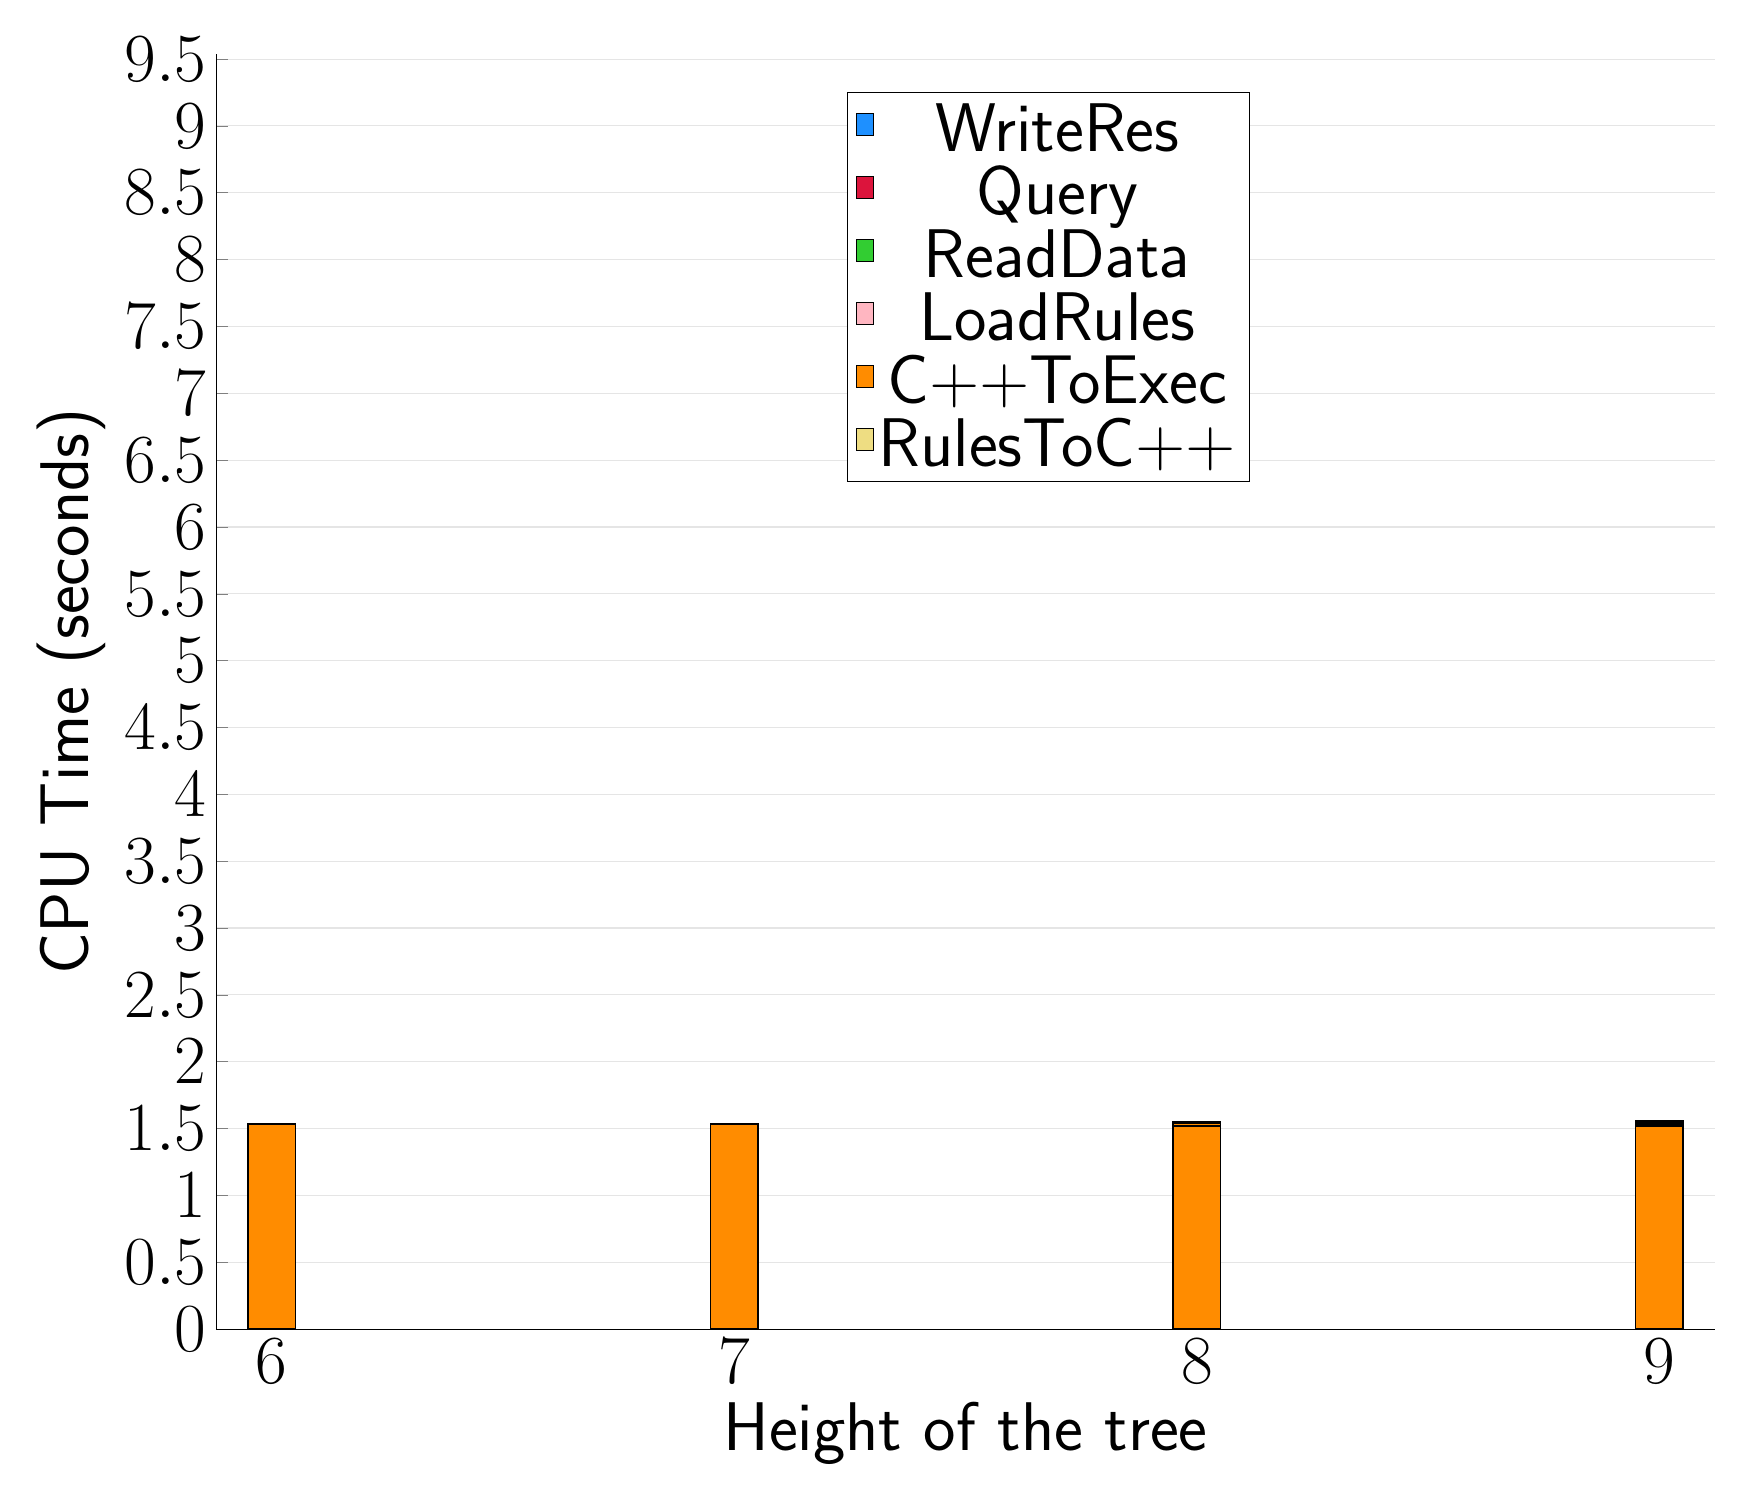
\begin{tikzpicture}
\begin{axis}[
   ybar stacked,
   width=1.7\textwidth,
   bar width=0.6cm,
   ymajorgrids, tick align=inside,
   major grid style={draw=gray!20},
   xtick=data,
   ymin=0, ymax=9.54,
   axis x line*=bottom,
   axis y line*=left,
   enlarge x limits=0.04,
   legend style={
       at={(0.69, 0.97)},
       anchor=north east,
       legend columns=1,
       font=\Huge,
   },
   ylabel={CPU Time (seconds)},
   xlabel={Height of the tree},
   label style={font=\Huge},
   tick label style={font=\Huge},
]
\addlegendimage{fill=DodgerBlue, draw=black, line width=0.2pt}
\addlegendentry{WriteRes}
\addlegendimage{fill=Crimson, draw=black, line width=0.2pt}
\addlegendentry{Query}
\addlegendimage{fill=LimeGreen, draw=black, line width=0.2pt}
\addlegendentry{ReadData}
\addlegendimage{fill=LightPink, draw=black, line width=0.2pt}
\addlegendentry{LoadRules}
\addlegendimage{fill=DarkOrange, draw=black, line width=0.2pt}
\addlegendentry{C++ToExec}
\addlegendimage{fill=LightGoldenrod, draw=black, line width=0.2pt}
\addlegendentry{RulesToC++}
\addplot +[fill=LightGoldenrod, draw=black, line width=0.55pt] coordinates {
(6, 0.0)
(7, 0.0)
(8, 0.0020000000000000005)
(8, 0.0)
(8, 0.0)
(9, 0.0)
(9, 0.0)
(9, 0.0020000000000000005)
(9, 0.0)
(9, 0.0)
};
\addplot +[fill=DarkOrange, draw=black, line width=0.55pt] coordinates {
(6, 1.5340000000000003)
(7, 1.5340000000000003)
(8, 1.538)
(8, 1.5240000000000002)
(8, 1.514)
(9, 1.52)
(9, 1.5219999999999998)
(9, 1.5259999999999998)
(9, 1.522)
(9, 1.54)
};
\addplot +[fill=LightPink, draw=black, line width=0.55pt] coordinates {
(6, 0.0001526)
(7, 0.00016979999999999998)
(8, 0.00016599999999999997)
(8, 0.0001718)
(8, 0.0001562)
(9, 0.00015460000000000002)
(9, 0.000154)
(9, 0.00016099999999999998)
(9, 0.0001696)
(9, 0.0001652)
};
\addplot +[fill=LimeGreen, draw=black, line width=0.55pt] coordinates {
(6, 0.0006948)
(7, 0.0010072)
(8, 0.0013593999999999998)
(8, 0.0014966)
(8, 0.001291)
(9, 0.0023084)
(9, 0.0023484)
(9, 0.0024034)
(9, 0.002422)
(9, 0.0023028)
};
\addplot +[fill=Crimson, draw=black, line width=0.55pt] coordinates {
(6, 0.0013587999999999999)
(7, 0.0036991999999999997)
(8, 0.0078554)
(8, 0.0083084)
(8, 0.0075868)
(9, 0.0173326)
(9, 0.017692400000000004)
(9, 0.017360800000000003)
(9, 0.0175328)
(9, 0.0167804)
};
\addplot +[fill=DodgerBlue, draw=black, line width=0.55pt] coordinates {
(6, 0.0004954)
(7, 0.0005788000000000001)
(8, 0.000377)
(8, 0.00042100000000000004)
(8, 0.0003644)
(9, 0.000394)
(9, 0.00037160000000000003)
(9, 0.00037759999999999996)
(9, 0.00034339999999999994)
(9, 0.0003856)
};
\end{axis}
\end{tikzpicture}

\end{document}
